\section{Zielsetzung}
\label{sec:Zielsetzung}

Im Versuch 353 wird das Relaxationsverhalten eines RC-Schwingkreises untersucht. 
Die RC-Konstante des Kreises soll mithilfe des an einem Oszilloskop gemessenen Spannungsabfalls bestimmt werden.
Außerdem soll die Frequenzabhängigkeit der Kondensatorspannungsamplitude in einem RC-Kreis untersucht werden.

\section{Theorie}
\label{sec:Theorie}


Wenn ein System aus seinem Ausgangszustand ausgelenkt wird und es nicht-oszillatorisch wieder in diesen zurückkehrt, 
wird dies als Relaxation bezeichnet. Die Änderungsrate der betrachteten Größe $A$ ist meist proportional zur Abweichung des Endzustandes $A(\infty)$
\begin{equation}\label{eq:relaxationsrate}
    \frac{\symup{d}A}{\symup{d}t} = c\left[A(t) - A(\infty)\right].
\end{equation}
Integriert vom Zeitpunkt 0 bis zum Zeitpunkt t ergibt sich 
\begin{equation}\label{eq:int_A}
    \int_{A(0)}^{A(t)} \frac{\symup{d}A'}{A' - A(\infty)} = \int_{0}^{t} c\symup{d}t' .
\end{equation}
%\begin{equation*}
%    \ln\left(\frac{A(t) - A(\infty)}{A(0) - A(\infty)}\right) = c t .
%\end{equation*}
Die Gleichung \eqref{eq:int_A} nach $A(t)$ aufgelöst ist
\begin{equation*}
    A(t) = A(\infty) + \left[A(0) - A(\infty)\right]\, \symup{e}^{\left(c t\right)}
\end{equation*}
gültig mit $c < 0$.
\\
\subsection{Kondensator}
Konkret betrachtet wird der Be- und Entladungsprozess eines Kondensators über einen Widerstand.
Für die Spannung an einem Kondensator gilt
\begin{equation}\label{eq:U_C}
    U_C = \frac{Q}{C}.
\end{equation}
Mit den Ohmschen Gesetzen ergibt sich der Strom
\begin{equation}\label{eq:I} 
    I = \frac{U_C}{R}.
\end{equation}

Die zeitliche Änderung der Kondensatorladung $Q$ ist durch die Gleichung
\begin{equation}\label{eq:Idt}%Hier ist dQ = Idt
    \symup{d}Q = -I\symup{d}t
\end{equation}
gegeben. Mithilfe der Gleichungen \eqref{eq:U_C} und \eqref{eq:I} wird diese Gleichung in die Form von \eqref{eq:relaxationsrate} gebracht
\begin{equation*}
    \frac{\symup{d}Q}{\symup{d}t} = -\frac{1}{RC}Q(t),
\end{equation*}
wobei $Q(\infty) = 0$ gilt.\\
Mit einer Integration wie in \eqref{eq:int_A} ist 
\begin{equation*}\label{eq:Q}%irgendwie stimmen hier die Größen von Q und e optisch nicht zueinander
    Q(t) = Q(0)\, \symup{e}^{-\frac{t}{RC}}.
\end{equation*}
\\
%Aufladevorgang
Mit den Randbedinungnen $Q(0) = 0$ und $Q(\infty) = CU_0$
wird der Aufladevorgang durch die Gleichung 
\begin{equation*}\label{eq:Kondensatoraufladung}
    Q(t) = CU_0\left(1 - \symup{e}^{-\frac{t}{RC}}\right)
\end{equation*}
beschrieben. Unter Verwendung von \eqref{eq:U_C} kann die Gleichung umgeformt werden zu
\begin{equation*}\label{eq:RC}
    \ln{\left(\frac{U_C}{U_0}\right)} = -\frac{t}{RC}.
\end{equation*}
Wird der $\ln{\left(\frac{U_C}{U_0}\right)}$ gegen die Zeit $t$ aufgetragen ergibt der
negative Kehrwert der Steigung die RC-Konstante.\\
%\begin{equation*}
%    \frac{Q(t = RC)}{Q(0)} = \frac{1}{\symup{e}} \approx 0.368.
%\end{equation*}
\subsection{Relaxationsphänomene bei periodischer Auslenkung}
Unter sinusförmiger periodischer Auslenkung zeigen sich auch Relaxationsphänomene.
Ist die Kreisfrequenz $ω$ des Auslenkungssignals 
\begin{equation*}
    U(t) = U_0 \cos{\left(\omega t\right)}
\end{equation*}
ausreichend klein, also $ω<<\frac{1}{RC}$, so ist die Kondesatorspannung $U_C(t)$ jederzeit gleich $U(t).$
Mit steigender Frequenz verschiebt sich der Be- und Entladevorgang des Kondensators immer weiter hinter den Verlauf der Generatorspannung.
Die Amplitude $A$ der Kondensatorspannung nimmt ab und es bildet sich eine Phasenverschiebung $φ$ zwischen den Spannungen aus.
Um die Frequenzabhängigkeit der Phase und Amplitude von $U_C$ herauszufinden eignet sich der Ansatz
\begin{equation}\label{eq:U_C_phi}
    U_C(t) = A(ω) \cos{\left(ωt +  φ\{ω\}\right)}.
\end{equation}
\begin{figure}[h]
    \centering
    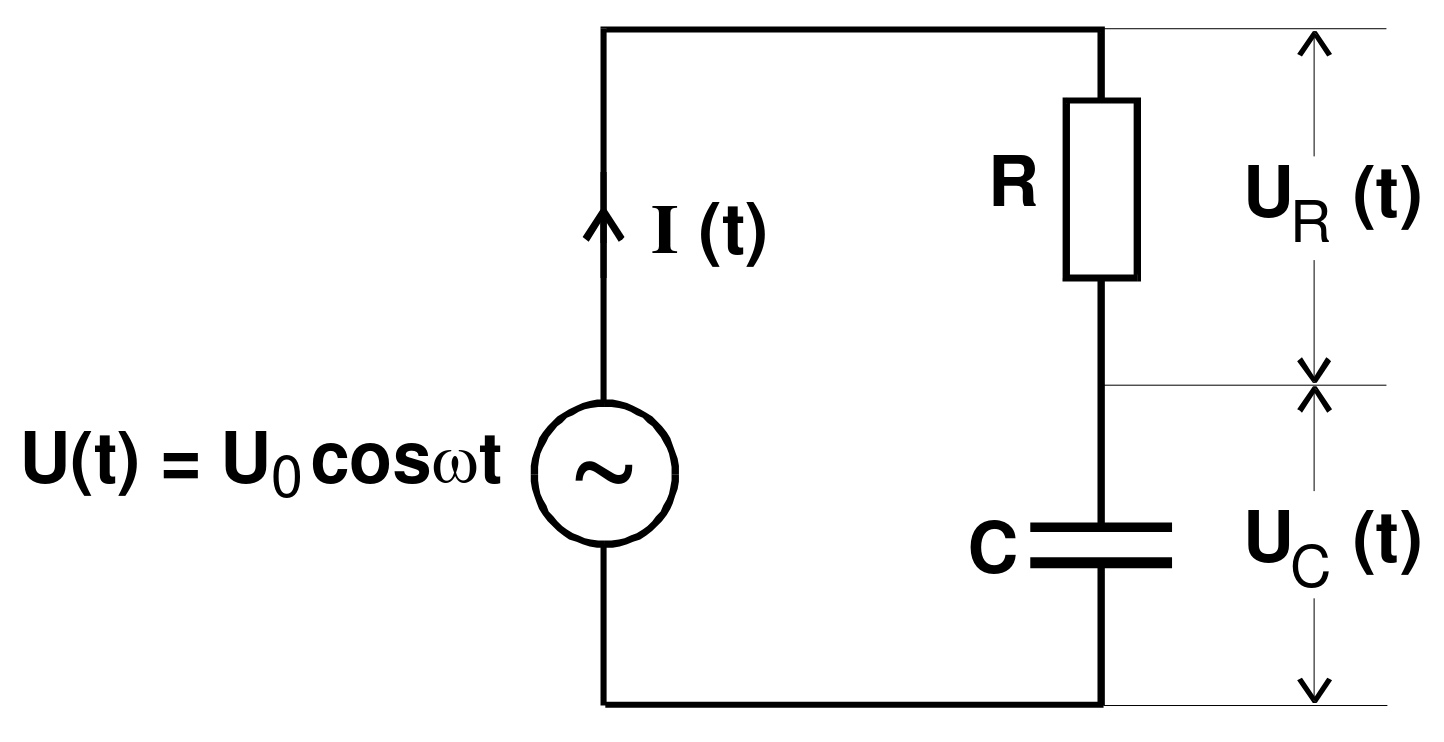
\includegraphics[width=0.5\textwidth]{img/kirchhoff.png}
    \caption{Beispielhafte Schaltskizze eines RC-Schwingkreises.\cite{V353}}
    \label{fig:Kirchhoff}
\end{figure}
\newpage
Aus einer Schaltung wie in \autoref{fig:Kirchhoff} lässt sich mithilfe des zweiten Kirchhoffschen Gesetzes folgender Ausdruck für die Gesamtspannung herleiten
\begin{equation}\label{eq:Uges}
    U(t) = U_R(t) + U_C(t),
\end{equation}
ausformuliert wird die Gleichung zu
\begin{equation}\label{eq:KirchhoffAusformuliert}
    U_0\cos{ωt} = I(t)R + A(ω)\cos{\left(ωt +  φ\right)}.
\end{equation}
Die Gleichung ist nur unter der Voraussetzung gültig, dass der Innenwiederstand $R_{\symup{i}} = 0$ ist,
da sonst $U_R(t) = (R + R_{\symup{i}})\cdot I(t).$\\
Der Strom $I(t)$ lässt sich mit Gleichung \eqref{eq:U_C} und \eqref{eq:Idt} umformulieren zu
\begin{equation}\label{eq:Strom_I}
    I(t) = \frac{\symup{d}Q}{\symup{d}t} = C\frac{\symup{d}U_C}{\symup{d}t}.
\end{equation}
Zusammen mit den Gleichungen \eqref{eq:U_C_phi}, \eqref{eq:KirchhoffAusformuliert} und \eqref{eq:Strom_I} ergibt sich
\begin{equation}\label{eq:keinPlan}
    U_0\cos{ωt} = -AωRC\sin{\left(ωt + φ\right)} + A(ω)\cos{\left(ωt + φ\right)}.
\end{equation}
Die Gleichung \eqref{eq:keinPlan} muss für jedes t gelten.\\
Für $ωt = \frac{π}{2}$ gilt dann
%\begin{equation*}
%    0 = -ωRC\sin{\left(\frac{π}{2} + φ\right)} + \cos{\left(\frac{π}{2} + φ\right)}
%\end{equation*}
%daraus folgt wegen $\sin{\left(φ + \frac{π}{2}\right)} = \cos{φ}$ und $\cos{\left(φ + \frac{π}{2}\right)} = -\sin{φ}$
\begin{equation}\label{eq:phi}
    \frac{\sin{φ}}{\cos{φ}} = \tan{φ (ω)} = -ωRC \quad \text{oder} \quad φ(ω) = \arctan{\left(-ωRC\right)}.
\end{equation}
Für hohe Frequenzen geht $φ$ also asymptotisch gegen $\frac{π}{2}$, für niedrige Frequenzen gegen $0$.\\
Bei $ω = \frac{1}{RC}$ ist $φ = \frac{π}{4}.$
Weiter folgt aus \eqref{eq:keinPlan} mit $ωt + φ = \frac{π}{2}$ die Gleichung
%\begin{equation*}
%    U_0\cos{\left(\frac{π}{2} - φ\right)} = -AωRC
%\end{equation*}
%beziehungsweise 
\begin{equation}\label{eq:A}
    A(ω) = -\frac{\sin{φ}}{ωRC}U_0.
\end{equation}
Aus Gleichung \eqref{eq:phi} kann %mit der Identität $\sin{φ}^2 + \cos{φ}^2 = 1$ die Beziehung
%\begin{equation*}
%    \sin{φ} = \frac{ωRC}{\sqrt{1 + ω^2R^2C^2}}
%\end{equation*}
%hergeleitet werden. Eingesetzt in \eqref{eq:A} folgt die Gleichung
\begin{equation}\label{eq:A2}
    A(ω) = \frac{U_0}{\sqrt{1 + ω^2R^2C^2}}
\end{equation}
hergeleitet werden.
Aus \eqref{eq:A2} lässt sich erkennen, dass die Amplitude $A(ω)$ für $ω\to 0$ gegen $U_0$ und für $ω\to \infty$ gegen $0$ geht.
Bei einer Kreisfrequenz von $\frac{1}{RC}$ ist $A = \frac{U_0}{\sqrt{2}}.$
\newpage
\subsection{RC-Kreis als Integrator}
Zeitlich veränderliche Spannungen die wie in \autoref{fig:Kirchhoff} an einem Kondensator anliegen, können unter bestimmten Voraussetzungen durch einen RC-Kreis integriert werden.
%Ist die Frequenz $ω>>\frac{1}{RC}$, so ist die Spannung $U_C$ proportional zum Integral über die Zeit von $U(t)$.
%Mit der Gleichung \eqref{eq:Uges} ergibt sich für
%\begin{equation*}
%    U(t) = I(t) R + U_C(t).
%\end{equation*}
Die Gleichung \eqref{eq:Uges} mit $I(t)$ durch \eqref{eq:Strom_I} ersetzt ergibt
\begin{equation}\label{eq:Uges2}
    U(t) = RC\frac{\symup{d}U_C}{\symup{d}t} + U_C(t).
\end{equation}
Wird $ω >> \frac{1}{RC}$ angenommen so ist $\left\lvert U_C\right\rvert << \left\lvert U_R\right\rvert $
und $\left\lvert U_C\right\rvert << \left\lvert U\right\rvert $.
Dann kann \eqref{eq:Uges2} angenähert werden als
\begin{equation*}
    U(t) = RC\frac{\symup{d}U_C}{\symup{d}t}
\end{equation*}
oder als
\begin{equation*}
    U_C(t) = \frac{1}{RC} \int_{0}^{t} U(\tau)\symup{d}\tau.
\end{equation*}
Die Spannung $U_C(t)$ ist also proportional zum Integral über die Zeit von $U(t)$.
